
% This LaTeX was auto-generated from MATLAB code.
% To make changes, update the MATLAB code and republish this document.

\documentclass{article}
\usepackage{graphicx}
\usepackage{color}

\sloppy
\definecolor{lightgray}{gray}{0.5}
\setlength{\parindent}{0pt}

\begin{document}

    
    \begin{verbatim}
%Hw-3 Prb2
%Navneet Singh (nsingh1@andrew.cmu.edu)

%For scaling, we used $\theta = \frac{T}{T_F}$

function problem2
clc       %clear screen
clear all % clearing all stored variables
close all %close previous plots

%Given data
rho = 8933; %kg/m^3
d = 0.002; %m
sigma = 5.676e-8; %W/m^2K^4

%calculating constant term to be used in differential equation
a = 2*sigma/(rho*d);

t_star = 1; %sec, for scaling time
Tf = 1200; %K, furnance temperature
theta0 = 300/1200; %initial value for theta, scaled temperature

%defining ODE to be integrated
func = @(tau, theta) t_star*a*(Tf^3)*(1-theta^4)/(355.2 + 0.2008*Tf*theta);

tspan = [0 100]; %range of integration
[tau, theta] = ode45(func, tspan, theta0); %solving for theta

plot(tau, theta)
xlabel('$\tau$','interpreter','latex')
ylabel('$\theta$','interpreter','latex')
title('$\theta (\tau)$ Plot','interpreter','latex')


%Part (B)
%Following is the data showing density of copper 'rho' as a function of
%temperature. We will use non-linear regression to obtain relation density
%of copper as function of temperature.
T= [0.00,100.00,200.00,300.00,400.00,500.00,600.00,700.00,800.00,900.00,1000.00,1100.00,1200.00]; %K
rho=[9.08,9.04,9.00,8.96,8.91,8.87,8.82,8.76,8.71,8.65, 8.58,8.51,8.44]; %gm/cm^3

%defining the relation as rho = a*temp + b
rho_cu = @(a, T) a(1)*T+ a(2);
%making guess for the value of parameters
guess = [0, 9];
%using nlinfit function to get parameters a and b.
beta = nlinfit(T, rho, rho_cu, guess);

fprintf('Slope of fitted data = %f\n', beta(1))
%calculating density at 300K and 1200K
fprintf('Using data above, density at 300K = %f gm/cm^3\n',rho_cu(beta, 300))
fprintf('Using data above, density at 1200K = %f gm/cm^3\n',rho_cu(beta, 1200))

%As we can see slope of the fitted data is nearly zero, so density does't
%change much with the temperature. So our assumption was right.

end
\end{verbatim}

        \color{lightgray} \begin{verbatim}Slope of fitted data = -0.000528
Using data above, density at 300K = 8.953022 gm/cm^3
Using data above, density at 1200K = 8.477802 gm/cm^3
\end{verbatim} \color{black}
    
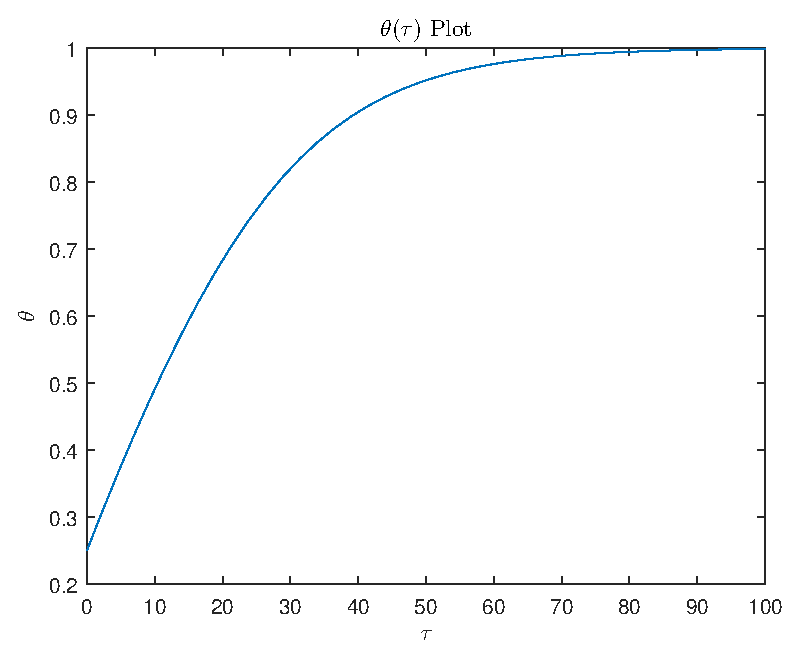
\includegraphics [width=4in]{problem2_01.eps}



\end{document}
    
